\chapter{Conclusions}

\section{Summary}

A measurement of the production of a {\PW} and a $\PZ$ boson in association with two jets has been presented,
using events where both bosons decay leptonically.
Results are based on data corresponding to an integrated luminosity of $35.9\fbinv$
recorded in proton-proton collisions at $\sqrt{s} = 13\TeV$ with the CMS detector
at the LHC in 2016. The cross section in a tight fiducial region with enhanced contributions from
electroweak (EW) \WZ production is $\sigma^{\mathrm{fid}}_{\WZjj} = 3.18^{+0.71}_{-0.63}\unit{fb}$,
consistent with the standard model (SM) prediction.
The dijet mass and dijet rapidity separation are used to measure
the signal strength of \EWWZ production with
respect to the SM expectation, resulting in
$\mu_{\EW} = 0.82^{+0.51}_{-0.43}$.
The significance of this result is
2.2 standard deviations with 2.5 standard deviations expected.
at $13\TeV$.
This is the first study of this process performed by the CMS Collaboration.

Constraints are placed on anomalous quartic gauge couplings
in terms of dimension-eight effective field theory operators, and
upper limits are given on the production cross section
times branching fraction of charged Higgs bosons.
The upper limits on charged Higgs boson production
via vector boson fusion with decay to a {\PW} and a {\cPZ} boson
extend the results previously published
by the CMS Collaboration~\cite{Sirunyan:2017sbn} and
are comparable to those of the ATLAS Collaboration~\cite{Aaboud:2018ohp}.
These are the first limits for dimension-eight effective field theory
operators in the \WZ channel at 13\TeV.

\section{Outlook}

The \WZjj and \EWWZ cross section measurements are statistically limited.
Therefore, a significant reduction in the uncertainty is expected from
analyzing a larger data set. The CMS experiment collected data from
13\TeV LHC collisions in 2017 and 2018, corresponding to data sets
of 41.1 and 59.7\fbinv of integrated luminosity.
By combining the results obtained here with
an analysis performed on this data set, sensitivity to the \EWWZ process
exceeding 5 standard is expected with only moderate
reductions in the systematic uncertainties. Differential measurements
of \WZjj production in variables sensitive to new physics and corrections from higher 
perturbative orders will also be possible with larger data sets.
A 50\% reduction in the total cross section uncertainty would be sensitive
to the large corrections NLO \EW corrections observed for the $\Wpm\Wpm$
VBS process~\cite{Biedermann:2016yds} and demonstrated in preliminary studies for \WZjj.
In addition, measurements with reduced uncertainties will definitively determine 
if the small degree of tension between this result and the result
recently submitted for publication by the ATLAS 
Collaboration~\cite{Aaboud:2018ddq} is a result
of statistical fluctuations or a consequence of different analysis
techniques or interpretations.

\begin{figure}[htbp]
  \centering
   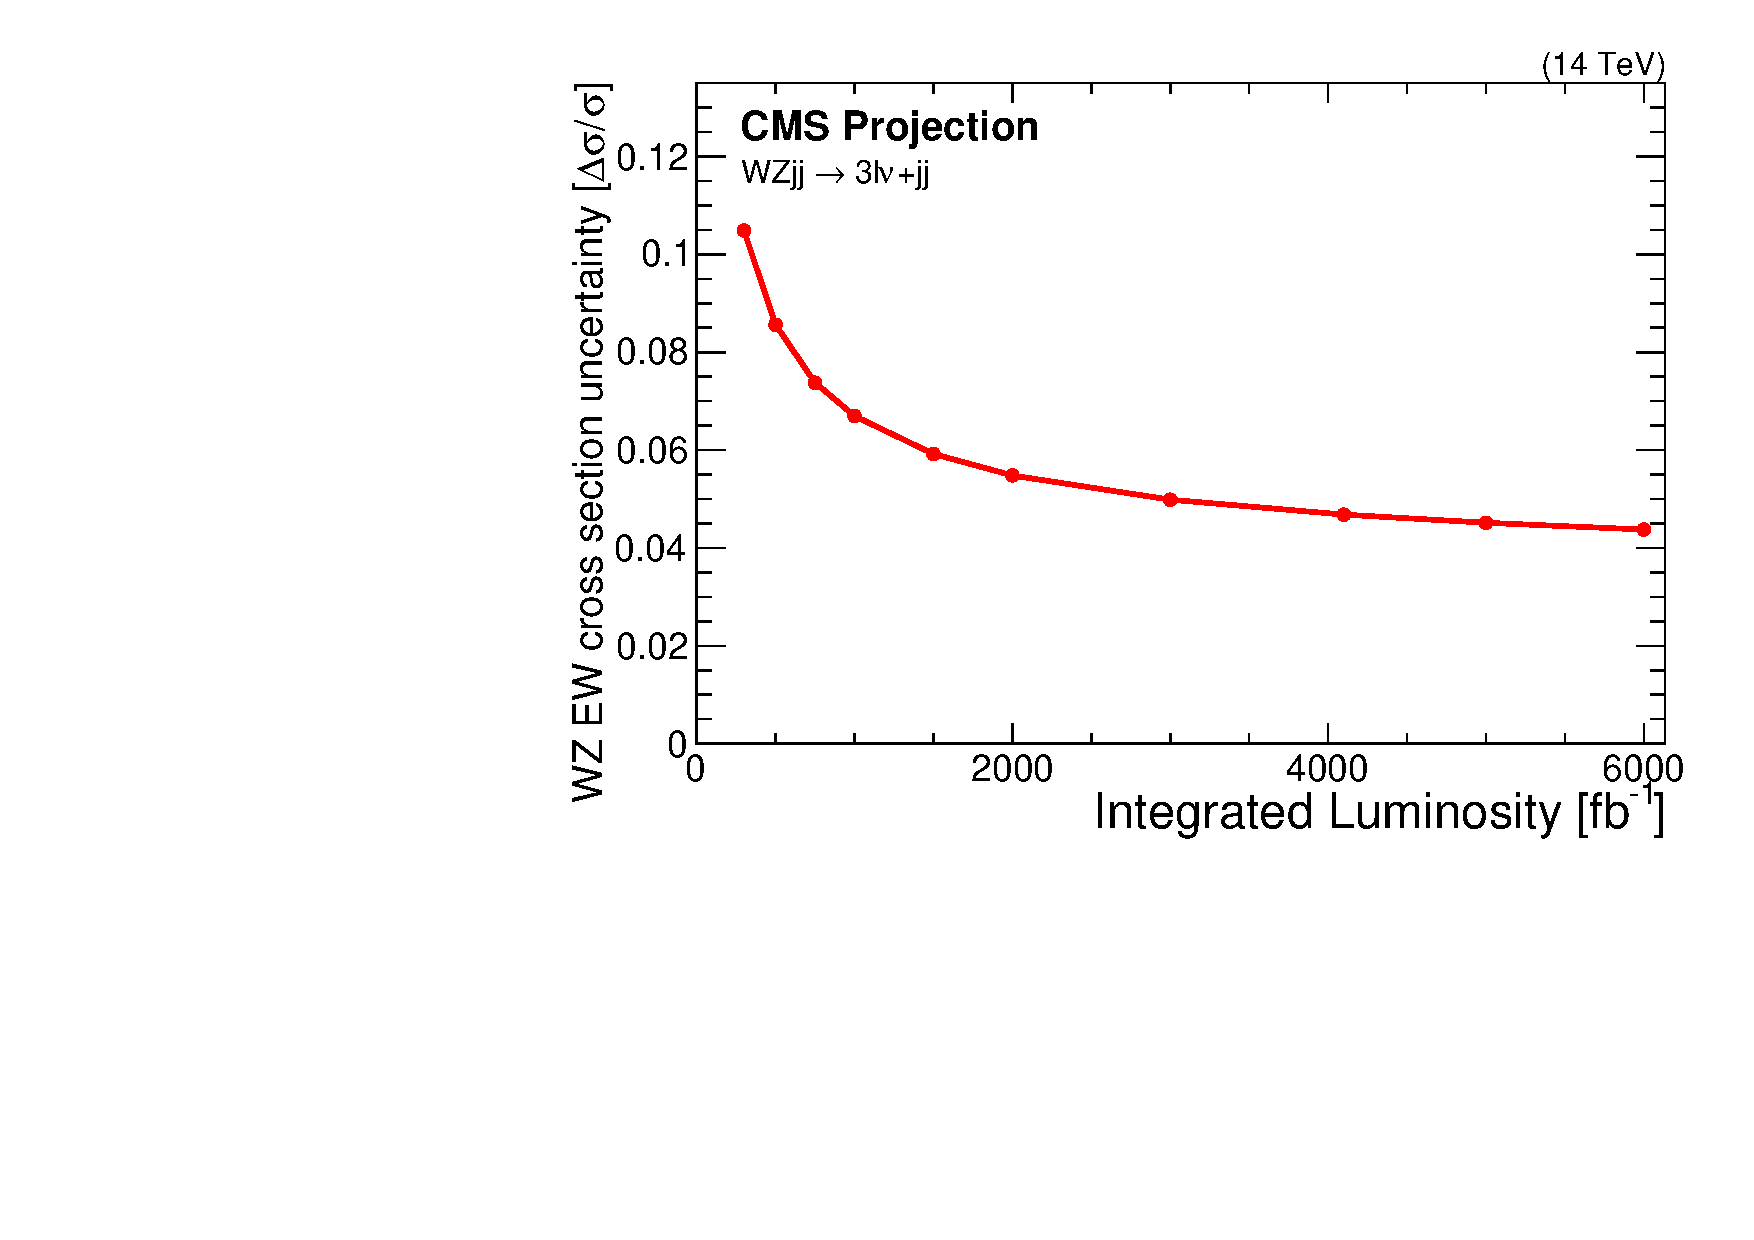
\includegraphics[width=0.6\textwidth]{figures/Conclusions/WZjjSignficanceHLLHC.pdf}
  \caption[Projected reduction in uncertainty for the \EWWZ cross section measurement at the HL-LHC]{
    Projected reduction in uncertainty for the \EWWZ cross section measurement 
    at the HL-LHC. Reproduced from Ref.~\cite{CMS-PAS-FTR-18-038}.
        }
 \label{fig:WZHLLHC}
\end{figure}

The data set collected by the CMS experiment in 2016-2018 constitutes only a small fraction
of the data expected to be delivered by the LHC in its lifetime. Beginning at the end of 2020, the LHC
will resume collisions, likely at an increased energy of 14\TeV. A data set corresponding
to 300\fbinv is expected to be collected by 2023, at which point the LHC will be upgraded to
deliver 5--7 times the current instantaneous luminosities with the high-luminosity LHC (HL-LHC).
During more than ten years of data taking the HL-LHC targets 3000\fbinv of data.
This analysis has been projected to the HL-LHC data set by extrapolating the 
luminosity and correcting estimating the change in reconstruction efficiency 
due to the harsh pileup conditions at the HL-LHC in Ref.~\cite{CMS-PAS-FTR-18-038}.
As shown in Figure~\ref{fig:WZHLLHC}, measurements of the \EWWZ process will be possible with
percent-level precision. In addition, sensitivity to the longitudinally polarized 
components of the \EWWZ process, which is closely linked to electroweak symmetry
breaking and is sensitive to spin-dependent new physics, may be observable 
by combining high-precision predictions with innovative analysis techniques.

Sensitivity to physics beyond the SM will also improve with the increasing LHC data set. 
The observable range of production cross sections 
and operator couplings is expected to improve proportional to the square root
of the luminosity, provided the systematic uncertainties remain subdominant.
Resonant production of massive particles requires a parton-parton interaction
with sufficient energy to produce the resonance, therefore,
the observable mass range of charged Higgs bosons or other charged
resonances would be dramatically improved by an increase in scattering energy.
A high-energy upgrade of the LHC (HE-LHC) that achieves \pp collisions at $\sqrt{s}=27\TeV$
by installing hypothetical 16\unit{T} magnets in the existing tunnel
has been proposed~\cite{Zimmermann:2647706}, following the completion of the 
HL-LHC project by 2040.
Ambitious proposals for a 100\TeV collider installed in a new 100\unit{km} tunnel at 
CERN or at a new location are also being considered~\cite{Mangano:2651294}.
It is almost universally accepted that new particles or interactions must exist between the electroweak scale 
set by $\sim m_{\PW} \sim m_{\PH}$ and the Planck Scale $\sim 10^{19}\GeV$,
however, unlike for the case of the Higgs boson and the LHC~\cite{RevModPhys.56.579}, 
a further restriction of this energy scale has not been convincingly established~\cite{Arkani-Hamed:2015vfh}.
With the current outlook for the field of particle physics, precision measurements, 
such as studies of the vector and Higgs boson couplings~\cite{Englert:2014uua,Anders:2018gfr}, 
remain exceedingly relevant.
Small deviations in observables sensitive to new interactions could point
to an energy scale of new particles, providing motivation and a target
energy regime for a new high-energy collider~\cite{Marciano_2002}. 
